\section{The Integration Algorithm}

The purpose of performing an intensity integration is 
to create a plot of average intensity as a function
of either $Q$, $2\theta$, or $\chi$. The algorithm
for performing an intensity integration is pretty
straight forward. In order to perform an intensity
integration, we must already know the calibration values
of the experiment for the particular image that will
be integrated. Than, a range and bin size for the
integration must be give. For example, you might
want to do a $Q-I$ integration from 2 to 5 with
100 bins. Whatever the range is, it 
must be specified before an integration is done.

The algorithm for performing the intensity integration
is as follows: loop over every pixel in the image. 
Add its intensity to the bin if it should be
in the bin based upon its value of $Q$, $2\theta$, or 
$\chi$. Remember that we need to use the calibration
values to calculate the corresponding $Q$, $2\theta$, and 
$\chi$ value using equation~\ref{ytermsydoubleprime}
\ref{xtermsxdoubleprime}, \ref{chitermsyx}, 
\ref{2thetatermsr}, and \ref{qterms2theta}.
After going through all the pixel, the bins then get averaged 
together. 

This program can constrain the integration. 
This means that you can perform, for example,
a $Q$ integration of only those pixels with some
particular range of $\chi$ values. Or, you can
constrain your $\chi$ integration to on a particular
$Q$ range. This could be used, for example, to
perform a $\chi$ integration of only a particular
diffraction peak. The algorithm for performing
the constraint isn't any more complicated. You just
only bin a particular intensity value if it is
allowed by the constraint.

Finally, the program can perform a polarization 
correction to the integration. The polarization 
correction formula is
\begin{align}
    I&=Im/PF \\ 
    PF&=P(1 - (\sin(2\theta)\sin(\chi-90))^2) + 
    (1 - P)(1 - (\sin(2\theta)\cos(\chi-90))^2)
\end{align}
with $Im$ the measured intensity. If this
is selected, what happens
then is that all pixels have their intensity
value corrected by this formula before they
are binned. Note that the $2\theta$ and $\chi$
values correspond to the particular value
that is being corrected.

\section{Integrating with the Program}


In order to perform a cake of the program you will have to 
already have loaded into the program one or more diffraction
data files and you will have to input calibration data
into the program. Figure~\ref{integration_page} shows the
\gui{Integrate} tab. This is where integration is done.
Notice that there are two separate inputs on the page. 
The input on the left is titled \gui{Q-I Integration}
and is for performing $Q$ integration.
The inputs on the left allow you to specify a
range in $Q$ that should be integrated.
The $Q$ range can be inputted with the
\gui{Q Lower?}, \gui{Q Upper?} inputs. The number of
bins in $Q$ space can be specified with the
\gui{Number of Q?} input. 
To perform a $Q$ integration, you have to push
the \gui{Integrate} button on the left.

\begin{SCfigure}[1][htb]
\centering
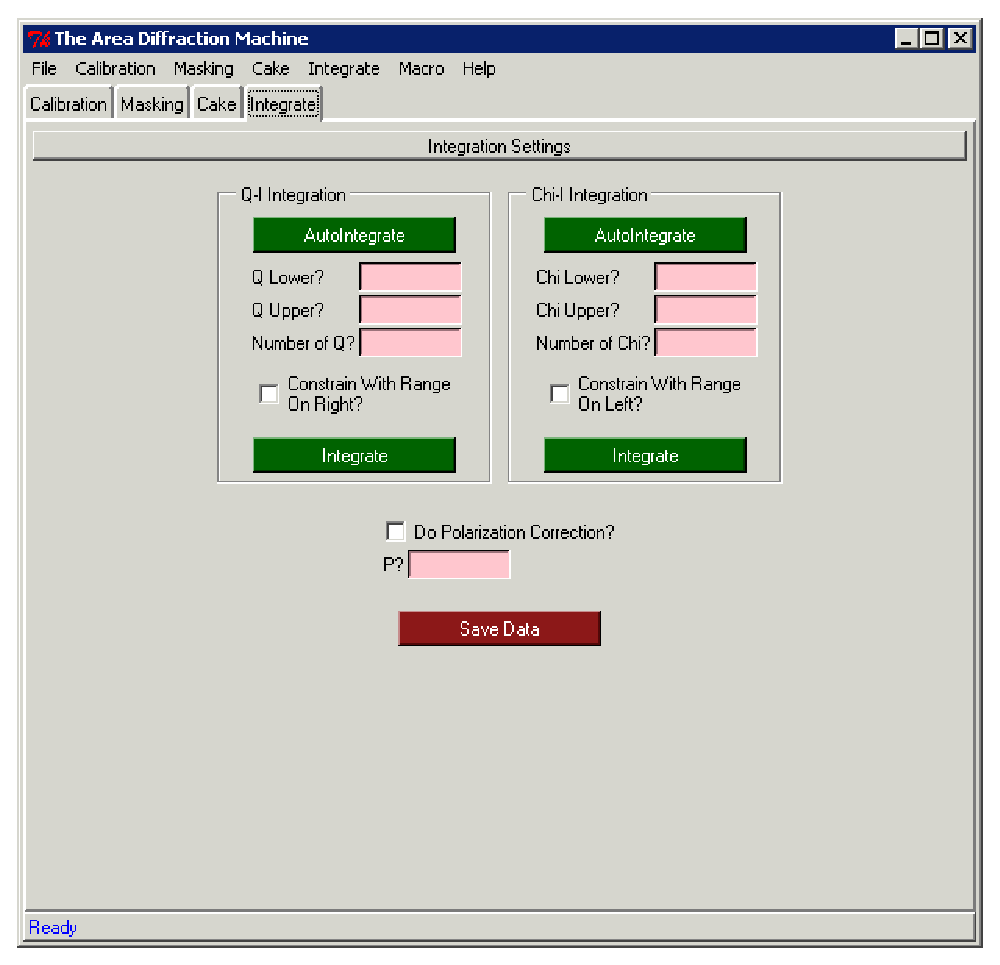
\includegraphics[scale=.75]{figures/integration_page.eps}
\caption{A screen shot of the integration tab to the 
    program. This is the tab where you can integrate data.} 
\label{integration_page}
\end{SCfigure}

To perform a $\chi$ integration, you can use the inputs
on the right under the name \gui{Chi-I Integration}.
The inputs on the right allow you to specify
a range in $\chi$ with the \gui{Chi Lower?} and
\gui{Chi Upper?} inputs. The number of bins in
$\chi$ space can be specified with the
\gui{Number of Chi?} input. To perform the
$\chi$ integration, you have to push the
\gui{Integrate} button on the right.

\section{The Integration Window}

\begin{SCfigure}[1][htb]
\centering
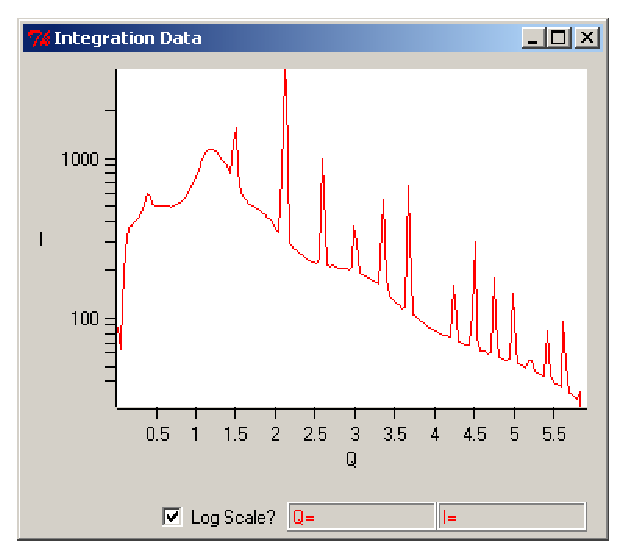
\includegraphics[scale=.75]{figures/integration_window_q.eps}
\caption{A screen shot of the integration window that
    opens up after you perform an intensity integration.} 
\label{integration_window_q}
\end{SCfigure}

\begin{SCfigure}[1][htb]
\centering
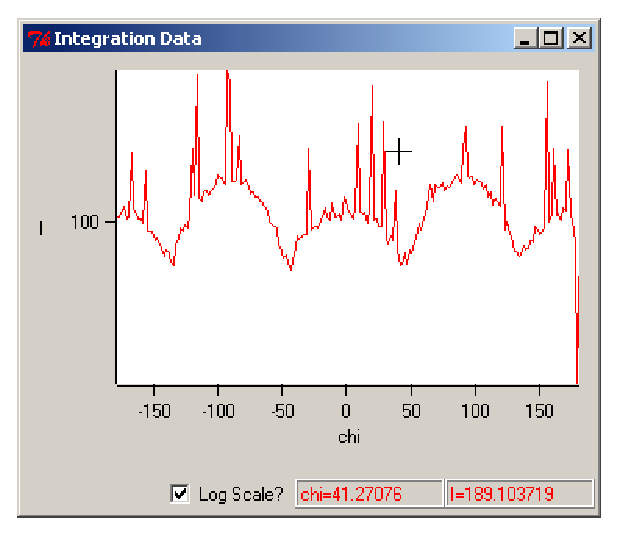
\includegraphics[scale=.75]{figures/integration_window_chi.eps}
\caption{A screen shot of the integration window that
    opens up after you perform an intensity integration.} 
\label{integration_window_chi}
\end{SCfigure}

After you push the integrate button, a line plot of the 
integrated data will be displayed in a new window. 
Figure~\ref{integration_window_q} shows 
the window displaying $Q$ integrated data
and figure~\ref{integration_window_chi} shows the
window displaying $\chi$ integrated ata.
Similar to the diffraction data display and the cake 
data display, this window has a couple of nice featuers
\begin{itemize}
    \item {\em Zoom into the data} - To zoom, left click
    on the data and hold down on the mouse. When you drag 
    the cursor, the program will create a resizing square. 
    When you let go of the mouse, the selected square will 
    be used as the outer bound and the image will be zoomed 
    into it. 
    \item {\em Zoom out of the data} - To unzoom, right
    click on the graph
    \item {\em Resize the window} - This will make the graph
    either larger or smaller. To do so, click on the bottom 
    right corner and drag. 
    \item {\em Read coordinates for a selected point} -
    When you mouse over the graph, the selected $Q$ (or $\chi$
    or $2\theta$) and intensity value will be displayed.
    \item {\em Log Scaling} - The \gui{Log Scale?} check box
    will toggle whether to display a log scale of the data.
\end{itemize}

\section{\texorpdfstring{Working in $2\theta$}{Working in 2theta}}

This program can integrate in $2\theta$ instead of $Q$. To 
do so, you have to go into menu bar up top and select
the \gui{Work in 2theta} option instead of the
\gui{Work in Q} option. Once you do this, the whole program
will just act like it was set to work in $2\theta$ all
along. The labels
on the program will change so that the option will say
\gui{2$\theta$-I Integration}. The other inputs will change
to \gui{2$\theta$ Lower}, \gui{2$\theta$ Upper}, and
\gui{Number of 2$\theta$}. When you push the left
\gui{Integrate} button, the program will integrate 
in $2\theta$ and the window that opens will show a plot
of average intensity as a function of $2\theta$.
If there are any values in the \gui{Q Lower} or
\gui{Q Upper}, they will be convert to $2\theta$
values when the program switches over. If you switch
from $2\theta$ back to $Q$, they will be converted
the other way.

\section{AutoIntegrate}

There is a convenience function similar to the
\gui{AutoCake} button called \gui{AutoIntegrate}. 
\gui{AutoIntegrate} will try to pick a nice range 
and then do the integration. The AutoIntegrate button 
on the left will guess at a nice range of $Q$ 
or $2\theta$ values and then do the $Q$ or
$2\theta$ integration.
It will always make the lower $Q$ or $2\theta$ 
value 0 and the upper value large enough
to include all the data.
It will set the number of $Q$ or $2\theta$ values to
200.

The \gui{AutoIntegrate} button on the right 
will guess a nice range of $\chi$ and then
do the $\chi$ integration. It will always 
set \gui{Chi Lower} to -180, \gui{Chi Upper} to
180, and \gui{Number of Chi} to 200.

\section{Constraining the Inputs}

As was described in the integration algorithm 
section, an integration in one parameter can 
be constrained by another parameter. For example,
a $Q$ or $2\theta$ integration can be done only 
of values in a particular $\chi$ range. Also,
A $\chi$ integration can be done only of a
particular $Q$ or $2\theta$ range. Of course,
it would be meaningless to constrain $Q$ by
$2\theta$.

To constrain the integration using the program,
there are two convenient 
\gui{Constrain With Range On Right?} and 
\gui{Constrain With Range On Left?} check boxes.
When you select
\gui{Constrain With Range On Right?}, the
$Q$ or $2\theta$ integration being done
will be constrained in $\chi$ by range
set with \gui{Chi Lower} and \gui{Chi Upper}.
When you select
\gui{Constrain With Range On Left?}, the
$\chi$ integration will be constrained by
either $Q$ or $2\theta$ (whichever mode the
program is currently in) by the lower and
upper inputs to the left.

\section{Masking}

The program can allows for masking of certain
pixels inside the image. 
Masking of intensity integrated data will be done
whenver the
\gui{Do Greater Than Mask?}, \gui{Do Less Than Mask?},
or \gui{Do Polygon Mask?} check boxes are selected.
Whenever the program finds an intensity value
that you specify should be masked (either because it 
is too large, too small, or in a polygon mask), it makes
sure not to bin that pixel and acts as though
it does not exist. So if you don't want to include
in your integration any values too large or too
small, you can use a threshold mask. If you
don't want to mask any values inside of a certain
region, you can use a polygon mask. 
Refer to Chapter \chapter{Pixel Masking}\label{pixel_masking}

When analyzing diffraction data, not all of the pixels in 
an image should be used in the analysis. In order to make 
the program ignore certain pixels, 
this program allows for two types of pixel masking:
threshold masking and polygon masking. You can 
apply either of these from the 
\gui{Masking} tab shown in  figure~\ref{masking_tab}.

\section{Threshold Masking}

\begin{SCfigure}[1][bthp]
    \centering
    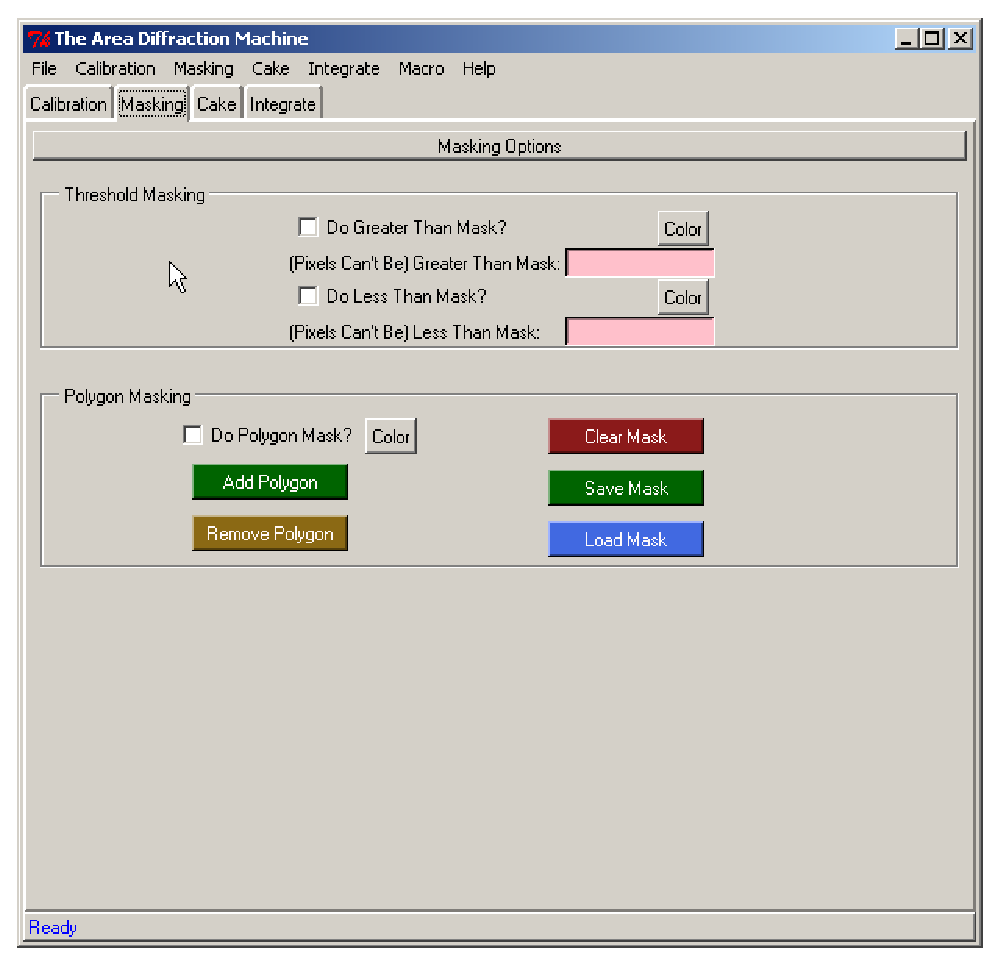
\includegraphics[scale=.75]{figures/masking_tab.eps}
    \caption{The pixel masking tab can be used to add
    a threshold mask or a polygon masking.} 
    \label{masking_tab}
\end{SCfigure}

The top half of the \gui{Masking} tab is devoted to 
threshold masking. Threshold masks allows all pixels, 
either above a certain intensity or below a certain 
intensity, to be ignored when doing the diffraction 
analysis. The \gui{Do Greater Than Mask?} check box can 
be used to apply a mask that will cause all pixels 
greater than a certain value to be ignored.
The \gui{(Pixel's Can't Be) Greater Than Mask} input 
can be used to specify the maximum pixel value.
The \gui{Do Less Than Mask} check box
can be used to make the program ignore all
pixels below a certain value. The particular value can 
be specified with the \gui{Less Than Mask} input. 

\begin{SCfigure}[1][bthp]
    \centering
    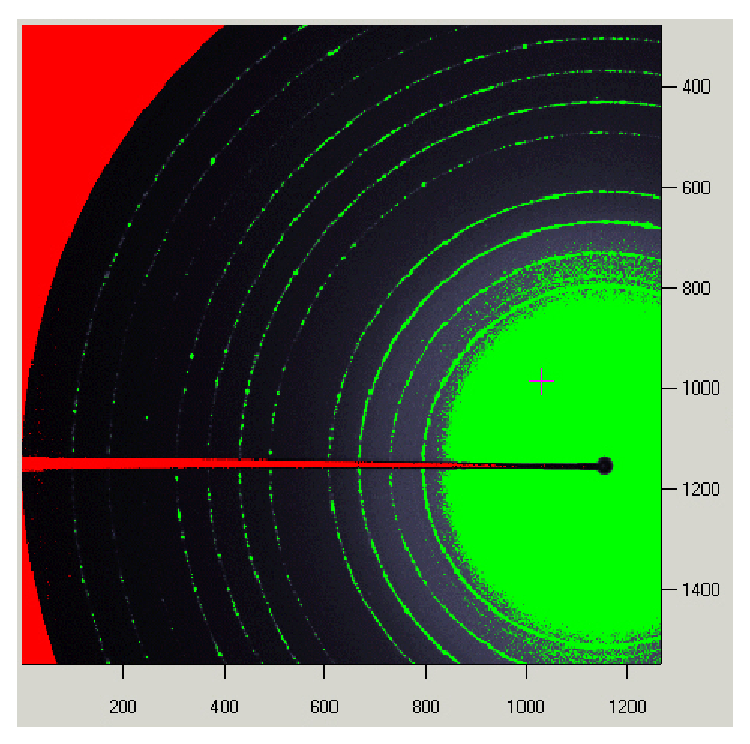
\includegraphics[scale=.75]{figures/Threshold_Masking.eps}
    \caption{A diffraction image with a
    greater than mask and less than mask.
    All pixels with intensity greater than 5000 
    have been colored green and all pixels with 
    intensity less than 30 have been colored red. Applying
    an intensity mask can be used to see if a detector's
    pixels have been overloaded. They can also be a used to
    ensure that overloaded pixels are not used in the
    data analysis.}
    \label{Threshold_Masking}
\end{SCfigure}

When applying a threshold mask, the pixels above or below
the threshold 
will be colored on the diffraction and cake image. 
The color can be set with the \gui{Color} button next to the greater 
than and less than masks. Figure~\ref{Threshold_Masking} shows 
diffraction image when all pixels
with intensity above 5000 are colored green and all pixels 
below 30 are colored red.

When caked data is saved, any of the pixels 
that are larger than the greater than mask are saved 
as -2. Any of the pixels smaller than the less than mask
are saved as -3. This behaviour needs to be accounted for
when analyzing caked data outside the program.

When an integrating intensity, 
any of the too high or too low pixels are simply ignored when 
calculating average intensity. 

\section{Polygon Masking}

Sometimes, large areas of a diffraction image should not
be included in the data analysis. For example, 
often a beam stop blocks part of the detector
and the pixels behind the beam stop should be ignored. 
This can be done with a polygon masks. Polygons can be drawn 
on the diffraction image and those parts 
of the image will not be used in subsequent analysis. 
This program can handle multiple polygons at the same time.

\begin{SCfigure}[1][bthp]
    \centering
    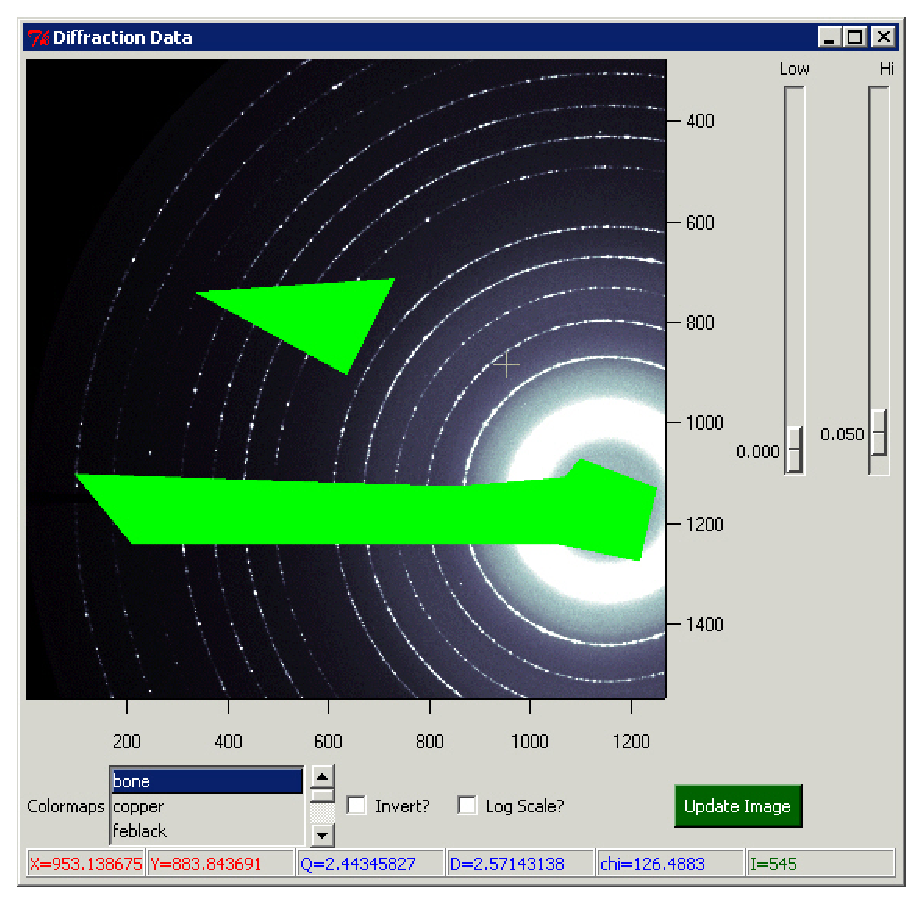
\includegraphics[scale=.75]{figures/Displayed_Polygon.eps}
    \caption{Two polygon masks that have been applied
    to this diffraction image. One of them covers the beam stop.}
    \label{Displayed_Polygon}
\end{SCfigure}

So long as the \gui{Do Polygon Mask?} check box is
selected, the polygon masks will be used 
when performing subsequent analysis. 
As figure~\ref{Displayed_Polygon} shows,
the polygons will be colored on the diffraction and
cake image.  The color of the polygon masks can be set 
with the \gui{Color} button
next to the \gui{Do Polygon Mask?} check box.
When caked data is saved, any pixels inside 
polygon masks will be given an intensity 
value of -4. During an intensity integration 
masked pixels will be ignored.

\begin{SCfigure}[1][bthp]
    \centering
    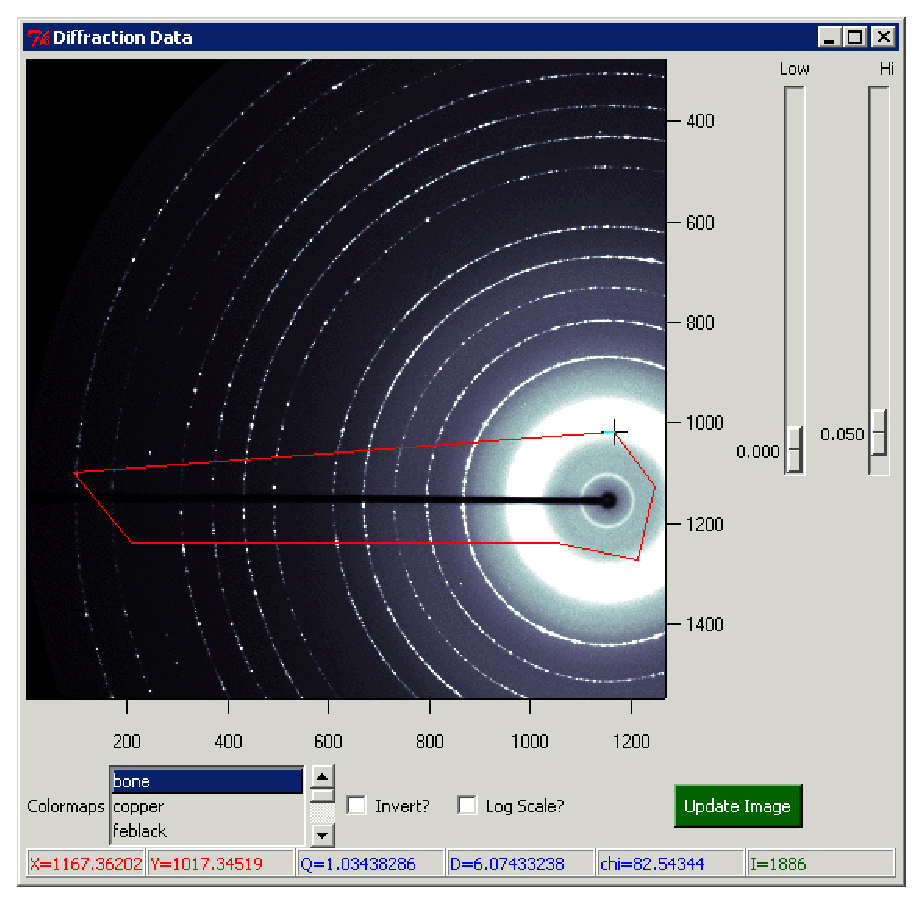
\includegraphics[scale=.75]{figures/Adding_Polygon.eps}
    \caption{A new polygon mask is being added to the 
    program. This particular mask will cover 
    the beam stop.}
    \label{Adding_Polygon}
\end{SCfigure}

A polygon mask can be added to the image with
the \gui{Add Polygon} button on the \gui{Masking} tab. 
This button will stay down when pushed and puts
the program in polygon drawing mode.  In this mode, the 
diffraction image can no longer be zoomed or panned.
Instead, left clicking on the diffraction image will make
the program draw a polygon mask.  The first left click adds the
first vertex. Each success left click add another vertex. 
The drawing can be finished and the final vertex added by right 
clicking. The program return to its
normal state and add the polygon into the program. 
Multiple polygons can be added using the \gui{Add Polygon}
button. Figure~\ref{Adding_Polygon} shows 
the program when a polygon is
being drawn. A half drawn polygon can be aborted without finishing
it by unpushing the \gui{Add Polygon} button.

\begin{SCfigure}[1][bthp]
    \centering
    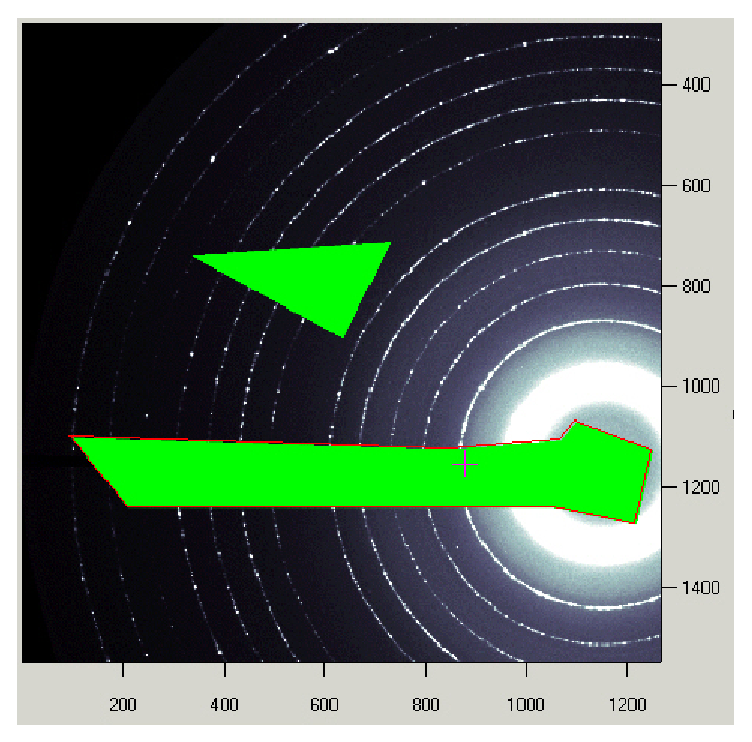
\includegraphics[scale=.75]{figures/Removing_Polygon.eps}
    \caption{A polygon is about to be removed.
    When mousing over a polygon to remove it,
    the program will display a red border around it.}
    \label{Removing_Polygon}
\end{SCfigure}

The \gui{Remove Polygon} button can be used to remove
a polygon from the program. Like the \gui{Add Polygon} 
button, this button will stay pushed and change the
behavior of the diffraction image. After pushing the 
\gui{Remove Polygon} button, clicking over
a particular polygon will remove it.
After the polygon is removed, the program will 
return to its normal state.
Figure~\ref{Removing_Polygon} shows what the diffraction
window looks like when a polygon is about to be removed.
The program can return to its normal state without
removing a polygon by unpushing the \gui{Remove Polygon}
button.

The \gui{Clear Mask} button can be used to remove
all the polygons at once. The \gui{Save Mask} button
can be used to save all the polygons to a file.
A file of polygons can be added to the program 
using the 
\gui{Load Mask} button. A polygon
file is very simple. The polygons in 
figure~\ref{Displayed_Polygon} were saved as
\begin{lstlisting}
# Polygon(s) drawn on Thu Feb 07 00:00:21 2008
93.140587183	1098.06704199
208.013978042	1237.77792276
1052.48863517	1237.77792276
1213.93231962	1271.92947139
1248.08386825	1126.00921814
1095.95424252	1067.02017959
1064.90738013	1104.27641447
847.579343365	1122.9045319

332.201427619	737.923438212
633.355992844	902.471808902
729.601266267	709.981262058
\end{lstlisting}
Each line is an ($x$,$y$) coordinate for one of 
the nodes of the polygon.  The coordinates are separated
by spaces. Each polygon is separated by a newline.  
Comment lines beginning with \# are 
ignored. 

\section{Masking Caked Plots}

Any polygon masks or threshold masks will also 
show up on the caked plot. As figure~\ref{box_mask} shows, 
polygons on a diffraction image can look very distorted on 
a caked plot. 

\begin{figure}[htb]
    \centering
    \subfloat[A rectangular polygon mask in 
    the middle of a diffraction image]{
    \label{box_mask_diffraction}
    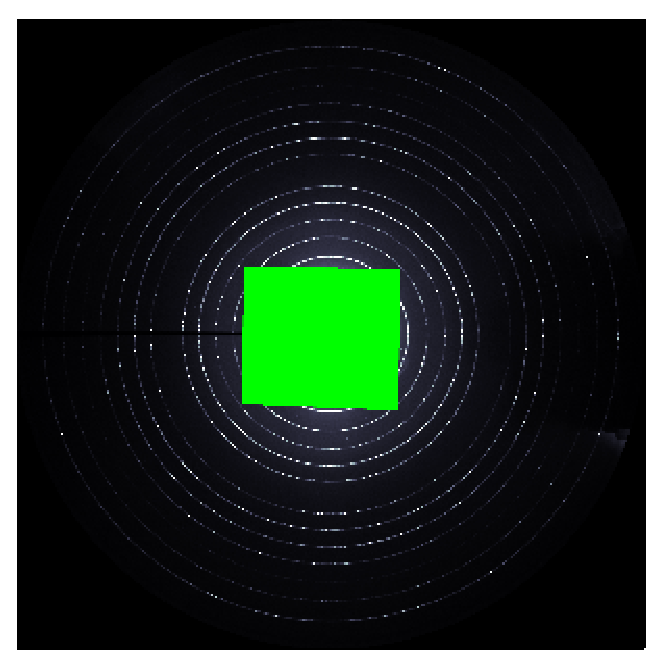
\includegraphics[scale=.7]
    {figures/box_mask_diffraction_image.eps}}\hspace{1em}
    \subfloat[The same rectangular mask on
    a caked plot]{
    \label{box_mask_cake}
    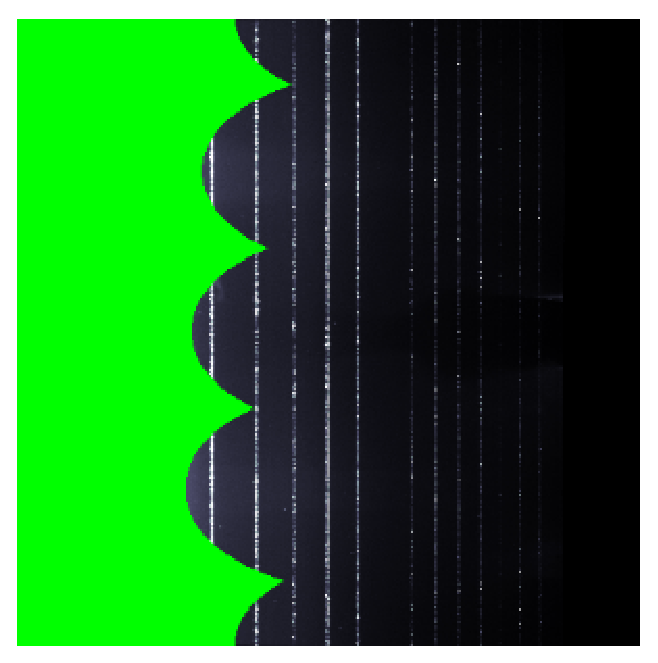
\includegraphics[scale=.7]{figures/box_mask_cake_image.eps}}
    \caption{A relatively simple shape on a diffraction image 
    can look very different on a caked plot.}
    \label{box_mask}
\end{figure}



 for information 
about how to apply a pixel mask.

\section{Saving Integrated Data}

After you have pushed the \gui{Integrate} buton
and performed a $Q$, $2\theta$, or $\chi$ integration,
you can save out the intensity integrated data
using the \gui{Save Data} button. The format of 
an intensity integration data file is as follows:
\begin{lstlisting}[caption={'The Cake Data Header'}]
# Q vs I Intensity Integration
# Intensity integration of: /Users/jolande/Desktop/LaB6_14_02_56.mar3450
# Data Integrated on Fri Mar 21 17:59:16 2008
# Calibration data used:
#   x center:    1725.0000000 pixels
#   y center:    1725.0000000 pixels
#   distance:     125.2960000 mm
#   energy:     12735.3957721 eV
#   alpha:          0.0000000 degrees
#   beta:           0.0000000 degrees
#   rotation:       0.0000000 degrees
#   pixel length:     100.0000000 microns
#   pixel height:     100.0000000 microns
# A polarization correction was applied
#   P = 1.000000
# A greater than mask was applied
#   Greater than mask = 10000.000000 (All pixels above 10000.000000 were ignored)
# A Less Than Mask was applied.
#   Less than mask = 50.000000 (All pixels below 50.000000 were ignored)
# Polygon mask(s) were applied
# Polygon(s) used in the analysis:
#   647.844364937	1369.72808587
#   1449.93738819	3226.88193202
#   2535.84794275	1449.93738819
#
#   1258.66905188	641.674418605
#   1215.47942755	999.531305903
#   1505.46690519	1116.76028623
#   1653.54561717	777.413237925
# Integration performed with a chi constraint
#   chi constraint lower: 90.000000
#   chi constraint upper: 270.000000
# Integration Range:
#   Q Lower = 0.000000
#   Q Upper = 6.726544
#   Number of Q = 200.000000
#   Q Step = 0.033633
# Q	Avg Intensity
0.016901	0.000000
0.050703	0.000000
0.084504	0.000000
0.118306	0.000000
0.152108	0.000000
0.185910	0.000000
\end{lstlisting}
The header is a bunch of lines that begin with #.
